% Measure original fig:exp5-m footprint at sigconf text width (for area evidence).
\documentclass[sigconf,nonacm]{acmart}
\usepackage{graphicx}
\usepackage{subfigure}
\settopmatter{printfolios=false,printccs=false,printacmref=false}
\graphicspath{{../../../tex/fig/panels/exp5/}}
\begin{document}
\thispagestyle{empty}
\begin{figure*}[t]
  \centering
  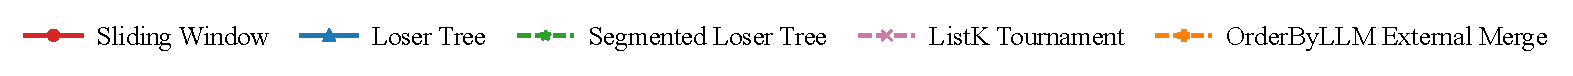
\includegraphics[width=0.8\linewidth]{exp5_legend.pdf}
  \vspace{-2ex}
  \subfigure[\Movies (full rank)]{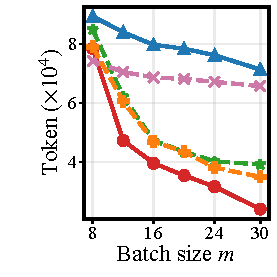
\includegraphics[width=0.33\columnwidth]{exp5_movies_full_tokens.pdf}}
  \hspace{-2.5ex}
  \subfigure[\Movies (full rank)]{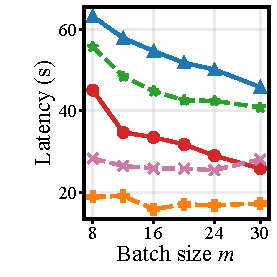
\includegraphics[width=0.33\columnwidth]{exp5_movies_full_latency.pdf}}
  \hspace{-2.5ex}
  \subfigure[\Movies (full rank)]{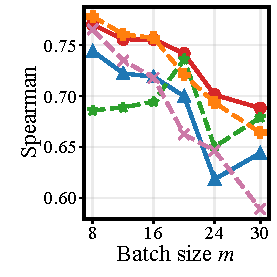
\includegraphics[width=0.33\columnwidth]{exp5_movies_full_quality.pdf}}
  \subfigure[\Movies (\LIMIT~$10$)]{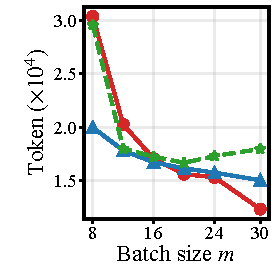
\includegraphics[width=0.33\columnwidth]{exp5_movies_top10_tokens.pdf}}
  \hspace{-2.5ex}
  \subfigure[\Movies (\LIMIT~$10$)]{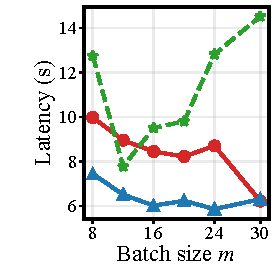
\includegraphics[width=0.33\columnwidth]{exp5_movies_top10_latency.pdf}}
  \hspace{-2.5ex}
  \subfigure[\Movies (\LIMIT~$10$)]{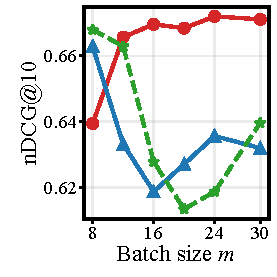
\includegraphics[width=0.33\columnwidth]{exp5_movies_top10_quality.pdf}}
  \subfigure[\DL20 (full rank)]{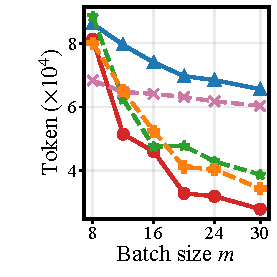
\includegraphics[width=0.33\columnwidth]{exp5_dl20_full_tokens.pdf}}
  \hspace{-2.5ex}
  \subfigure[\DL20 (full rank)]{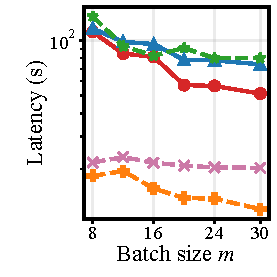
\includegraphics[width=0.33\columnwidth]{exp5_dl20_full_latency.pdf}}
  \hspace{-2.5ex}
  \subfigure[\DL20 (full rank)]{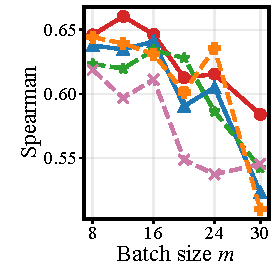
\includegraphics[width=0.33\columnwidth]{exp5_dl20_full_quality.pdf}}
  \subfigure[\DL20 (\LIMIT~$10$)]{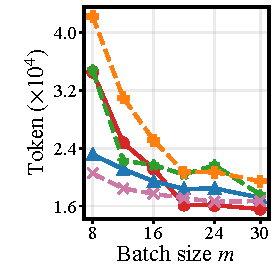
\includegraphics[width=0.33\columnwidth]{exp5_dl20_top10_tokens.pdf}}
  \hspace{-2.5ex}
  \subfigure[\DL20 (\LIMIT~$10$)]{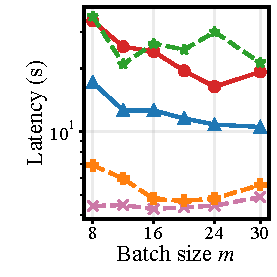
\includegraphics[width=0.33\columnwidth]{exp5_dl20_top10_latency.pdf}}
  \hspace{-2.5ex}
  \subfigure[\DL20 (\LIMIT~$10$)]{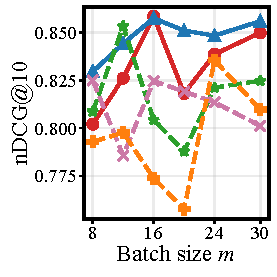
\includegraphics[width=0.33\columnwidth]{exp5_dl20_top10_quality.pdf}}
  \caption{Original \texttt{fig:exp5-m} container (reference footprint).}
\end{figure*}
\end{document}